\section{Methodology}
\label{sec:methodology}

This section describes the systematic literature review (SLR) protocol adopted to identify, screen, and synthesise the body of evidence concerning the use of Artificial Intelligence (AI) for risk mitigation in Supply Chain Management (SCM). The procedure was designed to ensure transparency, reproducibility, and methodological rigour throughout every stage of the review.

\subsection{Review Protocol}
\label{subsec:protocol}

The review followed the \textit{Preferred Reporting Items for Systematic Reviews and Meta-Analyses} (PRISMA) 2020 guidelines, which provide a structured framework for reporting the identification, screening, and inclusion of studies in systematic reviews.

The overarching goal of the protocol was to answer, in a systematic and reproducible manner, the following research questions (RQs):

\begin{itemize}
    \item \textbf{RQ1:} How can Artificial Intelligence be applied to mitigate risks in supply chains?
    \item \textbf{RQ2:} Which types of supply chain risks are addressed through AI-based approaches?
    \item \textbf{RQ3:} Which Artificial Intelligence techniques are employed for supply chain risk mitigation?
\end{itemize}

Each phase of the review---identification, screening, eligibility, and inclusion---was documented in accordance with the PRISMA 2020 flow diagram, allowing the entire selection process to be audited and replicated.

\subsection{Databases Searched}
\label{subsec:databases}

Two scientific databases were selected as primary sources for the literature search: \textbf{IEEE Xplore} and \textbf{Web of Science}.

The coverage period was restricted to publications released between \textbf{2019 and 2026}. This window was chosen to capture the most recent wave of AI adoption in SCM, including the period following major disruptions such as the COVID-19 pandemic and subsequent geopolitical shocks, which have substantially reshaped the academic discourse on supply chain resilience and risk.

\subsection{Search Queries}
\label{subsec:queries}

The search string was constructed along three conceptual dimensions: (i) the application \textit{domain} (Supply Chain), (ii) the \textit{technology} of interest (Artificial Intelligence and its synonyms), and (iii) the \textit{type of analysis} pursued (Risk Mitigation). Boolean operators were used to combine the dimensions, while quotation marks ensured exact-phrase matching. The final query is presented below:

\begin{center}
\texttt{"Supply Chain" AND ("Artificial Intelligence" OR "AI") AND "Risk Mitigation"}
\end{center}

The query was applied to the title, abstract, and keyword fields of both databases. Table~\ref{tab:queries} summarises the number of records retrieved per database.

\begin{table}
\centering
\caption{Number of records retrieved per database.}\label{tab:queries}
\begin{tabular}{|l|c|}
\hline
\textbf{Database} & \textbf{Records Retrieved}\\
\hline
IEEE Xplore & 142\\
Web of Science & 50\\
\hline
\textbf{Total} & \textbf{192}\\
\hline
\end{tabular}
\end{table}

The rationale behind combining these three dimensions was to balance \textit{recall"} (broad enough to capture different AI families, e.g., Machine Learning, Deep Learning, NLP) with \textit{precision} (narrow enough to filter out studies that, while mentioning AI or SCM, do not address the risk dimension explicitly).

\subsection{Screening Criteria}
\label{subsec:screening-criteria}

A first set of thematic filters was applied during the screening phase, that is, while reading the title, keywords, and abstract of each record. To advance beyond this stage, an article had to simultaneously satisfy the following three requirements:

\begin{enumerate}
    \item \textbf{Exclusive Supply Chain context.} The study had to demonstrate a practical application within logistics, procurement, inventory management, production planning, or transport networks. Articles addressing supporting technologies such as Blockchain or IoT from a purely technical perspective (e.g., network architecture or communication protocols), without applying them to logistics operations, were rejected.
    \item \textbf{Explicit presence of Artificial Intelligence.} Studies were required to employ advanced AI techniques, such as Machine Learning (ML), Neural Networks, Deep Learning (DL), Natural Language Processing (NLP), or genetic algorithms. Works limited to basic digitalisation, traditional automation, ERP systems, or the mere deployment of IoT/Blockchain sensors for data collection---without AI-based predictive or prescriptive processing---were excluded.
    \item \textbf{Central focus on risk prevention and mitigation.} The AI component had to be deployed in order to anticipate disruptions, manage market uncertainty (supply or demand), build resilience, foresee supplier failures, or minimise the impact of adverse events. Applications targeting strictly operational or commercial goals (e.g., optimising daily delivery routes or sales forecasting for marketing purposes), without a clear risk or resilience dimension, were excluded.
\end{enumerate}

\subsection{Eligibility Criteria}
\label{subsec:eligibility-criteria}

Articles that passed the screening phase were then subjected to a more demanding set of inclusion and exclusion criteria, applied during the full-text reading. The objective at this stage was no longer to identify articles broadly related to AI and Supply Chain, but to retain only studies offering a \textit{direct, substantive, and methodologically explicit} contribution to the research questions formulated in Section~\ref{subsec:protocol}.

\subsubsection{Inclusion Criteria.}
An article was retained only if it satisfied \textit{all} of the following requirements:

\begin{itemize}
    \item \textbf{IC1 --- Centrality of AI:} Artificial Intelligence had to be a central element of the article, rather than a peripheral or merely cited concept.
    \item \textbf{IC2 --- Risk-oriented purpose:} The main focus of the study had to be the mitigation, prediction, management, or assessment of risk in a supply chain context.
    \item \textbf{IC3 --- Methodological clarity:} The article had to describe explicitly (i) the AI techniques employed, (ii) the type(s) of risk addressed, and (iii) a concrete application, model, or methodology.
    \item \textbf{IC4 --- Tangible contribution:} The work had to present results, a framework, a model, an empirical study, or an applicable methodology.
    \item \textbf{IC5 --- Alignment with the RQs:} The article had to provide an explicit contribution to at least one of the three research questions (RQ1, RQ2, or RQ3).
    \item \textbf{IC6 --- Generalisability:} The context studied had to be sufficiently transferable to business and commercial supply chain settings.
\end{itemize}

\subsubsection{Exclusion Criteria.}
Conversely, an article was excluded whenever \textit{any} of the following situations occurred:

\begin{itemize}
    \item \textbf{EC1 --- Superficial use of AI:} AI mentioned without an underlying implementation or concrete methodology.
    \item \textbf{EC2 --- Operational focus without risk:} Primary emphasis on optimisation, efficiency, logistics, or operational performance with no clear link to risk mitigation.
    \item \textbf{EC3 --- AI as an accessory technology:} The article centres on digital transformation, Industry 4.0, IoT, Blockchain, or Big Data as its main theme, with AI playing only an ancillary role.
    \item \textbf{EC4 --- Unclear risk typology:} Failure to clearly identify the type(s) of supply chain risk being addressed.
    \item \textbf{EC5 --- Absence of a specific AI technique:} No specific AI model, algorithm, or method is described.
    \item \textbf{EC6 --- Excessive abstraction:} Overly conceptual or generic articles, lacking applicable results.
    \item \textbf{EC7 --- Out-of-scope risk:} The risk discussed is not genuinely a supply chain risk.
    \item \textbf{EC8 --- Limited transferability:} Studies confined to highly idiosyncratic contexts, whose findings cannot reasonably be generalised to broader business settings.
\end{itemize}

\subsection{Screening Process}
\label{subsec:screening}

The selection of studies was organised in three sequential phases, in line with the PRISMA 2020 flow.

\paragraph{Phase 1 --- Identification and removal of duplicates.}
The 192 records exported from IEEE Xplore and Web of Science were consolidated into a single reference manager. Three duplicate entries were identified and removed, resulting in 189 unique records advancing to the next stage.

\paragraph{Phase 2 --- Title, keywords, and abstract screening.}
Each remaining record was evaluated based on its title, keywords, and abstract, against the three thematic filters defined in Section~\ref{subsec:screening-criteria}. All three filters had to be simultaneously satisfied for an article to advance to the next phase. To ensure transparency and traceability, this stage was fully documented in a dedicated spreadsheet, in which each record was registered together with the following fields: \textit{Title}, \textit{Decision}, \textit{Risk Analysed}, \textit{AI Technique}, and \textit{Justification}. This structure made it possible to revisit individual decisions, audit the rationale behind each exclusion, and verify the consistency of judgements across the dataset. At the end of this phase, 128 records were removed (23 from IEEE Xplore and 105 from Web of Science), leaving 61 studies eligible for full-text assessment.

\paragraph{Phase 3 --- Full-text reading and eligibility assessment.}
The 61 surviving articles were retrieved in full and subjected to a stricter evaluation against the inclusion and exclusion criteria defined in Section~\ref{subsec:eligibility-criteria}. This phase was also documented in a structured spreadsheet, where each article was characterised through a richer set of descriptors aimed at supporting both the eligibility decision and the subsequent qualitative synthesis. For every record the following fields were registered: \textit{Title}, \textit{Authors}, \textit{Year}, \textit{Journal/Conference}, \textit{Country of the Authors}, \textit{Inclusion Criteria Satisfied}, \textit{Exclusion Criteria Triggered}, \textit{Decision}, \textit{Justification of the Decision}, \textit{AI Techniques}, \textit{Types of Risk Addressed}, \textit{Mitigation Approach}, \textit{Application Sector}, \textit{Type of Study}, \textit{Answer to RQ1}, \textit{Answer to RQ2}, \textit{Answer to RQ3}, \textit{Problem Addressed}, \textit{Main Contribution}, \textit{Limitations}, and \textit{Future Work}.

This extended template fulfilled a dual purpose. On the one hand, it operationalised the eligibility assessment by forcing an explicit mapping between each article and the inclusion and exclusion criteria, as well as the perceived strength of relevance (high, medium, or low). On the other hand, it already constituted the basis for the data extraction stage, since the AI techniques, risk types, mitigation approaches, and contributions per research question would later feed directly into the qualitative synthesis. A conservative posture was deliberately adopted: in cases of doubt, or whenever the methodological description of either the AI component or the risk dimension was insufficient, the article was excluded. Studies classified as having only \textit{low} relevance were likewise discarded, even when formally meeting the basic inclusion criteria.

Of the 61 articles assessed in this phase, 2 could not be retrieved in full text and 40 were excluded for failing to meet at least one of the criteria above, resulting in a final corpus of \textbf{19 studies} included in the qualitative synthesis.

\paragraph{Reviewer procedure.}
The screening and eligibility assessment were conducted as a team effort, with the set of articles distributed among the authors and evaluated individually against the criteria defined above. Each article was therefore reviewed by a single author, but the criteria, the spreadsheet templates, and the decision rubric were collectively defined and applied uniformly across the team. Borderline cases and decisions flagged as uncertain were brought to joint discussion and re-examined collectively, in order to ensure consistency of judgement across reviewers and to mitigate individual bias.

Figure~\ref{fig:prisma} summarises the full selection process, from the 192 records initially identified to the 19 studies retained for analysis.

\begin{figure}[H]
\centering
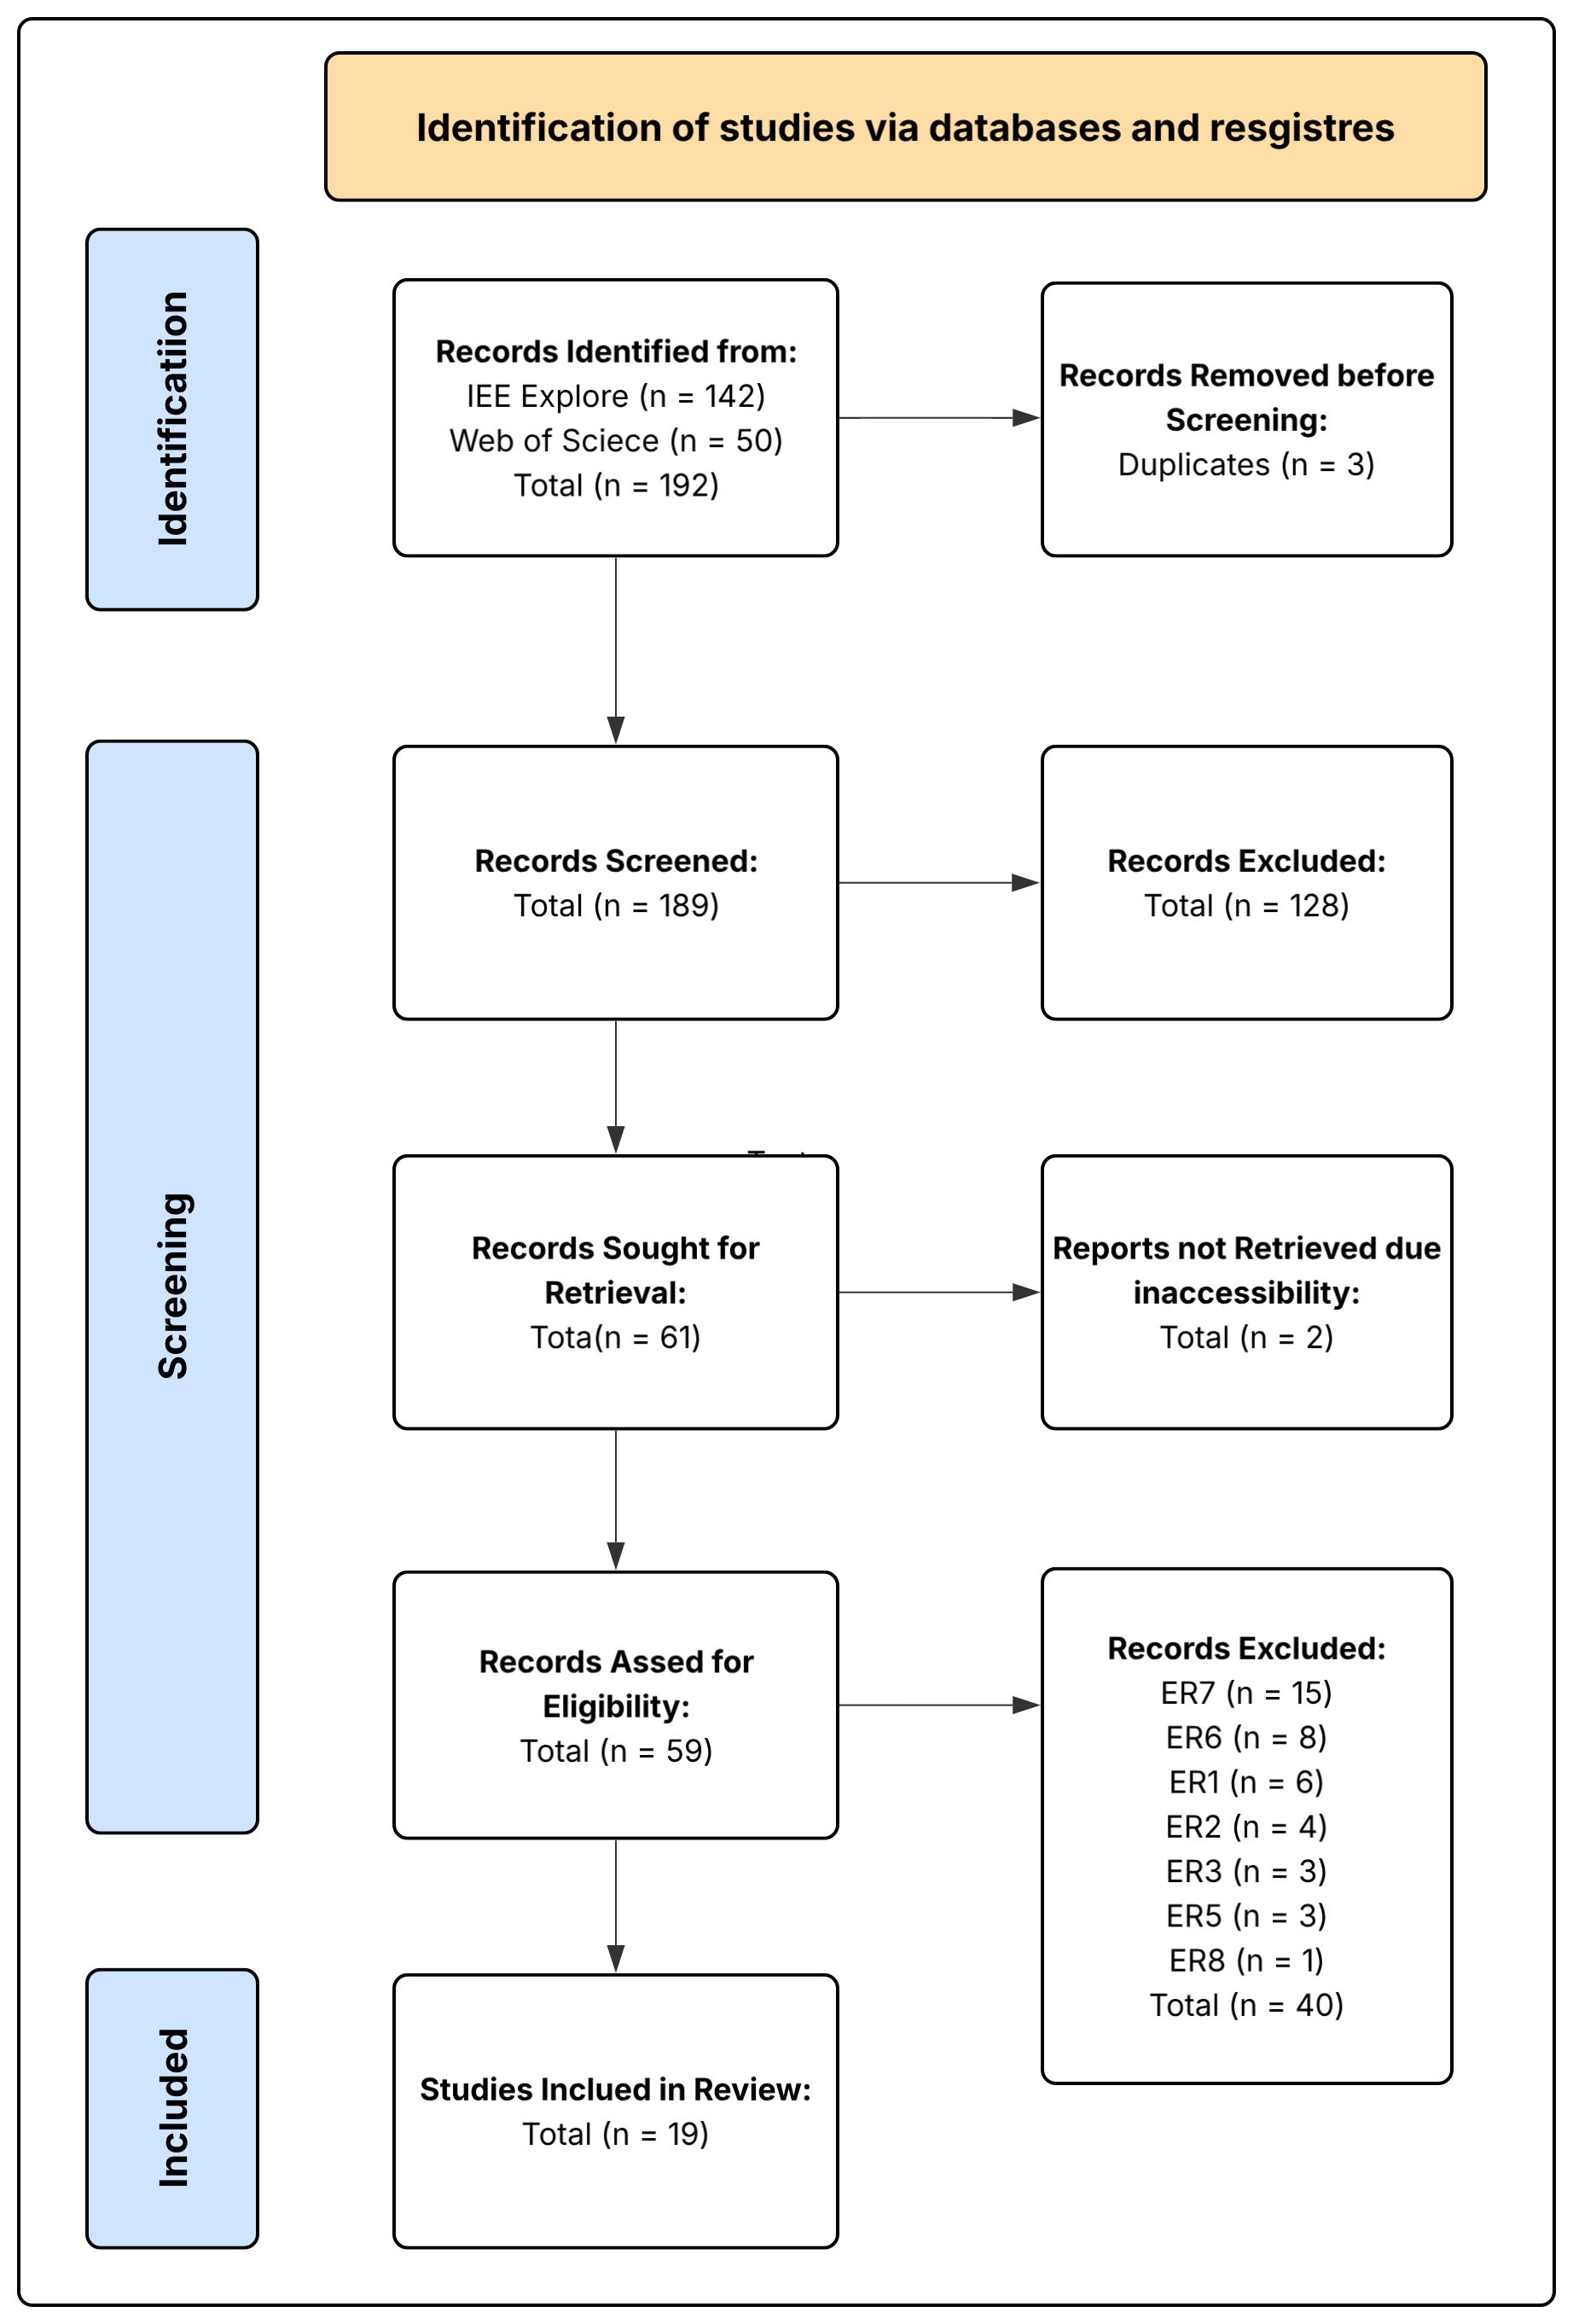
\includegraphics[width=\textwidth]{figures/prisma_flow_diagram.png}
\caption{PRISMA 2020 flow diagram of the study selection process.}\label{fig:prisma}
\end{figure}